\documentclass{IEEEcsmag}

\usepackage[colorlinks,urlcolor=blue,linkcolor=blue,citecolor=blue]{hyperref}

\usepackage{upmath}

\jvol{XX}
\jnum{XX}
\paper{8}
\jmonth{May/June}
\jname{Computing in Science and Engineering}
\pubyear{2021}
\newtheorem{theorem}{Theorem}
\newtheorem{lemma}{Lemma}

\setcounter{secnumdepth}{0}

\begin{document}

\sptitle{Department: Head}
\editor{Editor: Name, xxxx@email}

\title{PyExaFMM: Designing a highly-performant particle fast multipole solver in Python with Numba}

\author{\ S. Kailasa}
\affil{\ Department of Mathematics, University College London}

\author{\ T. Betcke}
\affil{\ Department of Mathematics, University College London}

\author{\ T. Wang}
\affil{\ Department of Mechanical and Aerospace Engineering, The George Washington University}

\author{\ L. A. Barba}
\affil{\ Department of Mechanical and Aerospace Engineering, The George Washington University}

\markboth{Department Head}{Paper title}

\begin{abstract}
PyExaFMM is a pythonic kernel-independent particle fast multipole method (FMM) implementation, built on the success of the ExaFMM project, to answer the question: can we develop a highly-performant scientific code without resorting to a lower level language? The FMM is a good case study to understand the maturity of Python in the development of high-performance software, due its reliance on a complex heirarchical octree data structure. In this paper we offer an overview the kernel-independent FMM algorithm and the mathematical and software development techniques we used in order to develop a performant practical implementation. We proceed to benchmark the software's accuracy, speed, and memory footprint with respect to the state of the art C++ implementation from the ExaFMM project. We report that we are able to achieve runtimes within $\mathcal{O}(10)$ of the state of the art, with comparable accuracy.

\end{abstract}

\maketitle

\chapterinitial{The introduction} What is the appeal of developing HPC codes in Python? Why is it a useful case-study, what does it mean. What is the FMM approximately, where is it used, why is it important? What will we talk about here, and what do we conclude? What will the remaining sections say?

\cite{Ying2004}

\section{THE KERNEL-INDEPENDENT FAST MULTIPOLE METHOD}

\subsection{Algorithm}

First introduced by Ying \cite{Ying2004}, the kernel-independent fast multipole method (KIFMM) \dots

\section{TECHNIQUES FOR ACHIEVING PERFORMANCE}

\subsection{What is Numba?}

What is does, how is it useful? Where do we use it, and why there. How much difference can it make in an idealized routine. What doesn't work, why doesn't it work. Where to be careful. Programming to an (invisible) framework \dots

Where is numba used heavily? Tree construction routines on Morton coordinates. Multithreading of tree construction, as well as P2M evaluation. Experiment to demonstrate the speed of kernel evaluation, with caveat that data must be pre-organised.

\subsection{Precomputing Operators}

Transfer vectors, hashing, HDF5, loading into memory.

\subsection{Compressing the M2L step with a randomised SVD}

Introduce \cite{Ying2004}. Numerical bounds on error out of scope, but show how experiments demonstrate that the FMM error dominates the SVD error.

\subsection{Software Architecture}

The key is separating routines to be accelerated, and organising data ready to run. The data organisation part (and it's slowness) should be demonstrated as a bottleneck using experiment.

\section{PERFORMANCE COMPARISON WITH STATE OF THE ART}

Description of main experiments, and how they are conducted. What are the main results? Are they expected from theory? What conclusions can be drawn about developing HPC codes entirely in Python, is it worth it?

\begin{figure}
\centerline{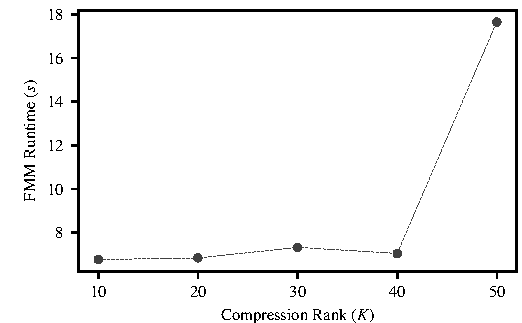
\includegraphics[width=18.5pc]{figures/compression_runtime.pdf}}
\caption{Compression Rank and runtime}
\end{figure}

\begin{figure}
\centerline{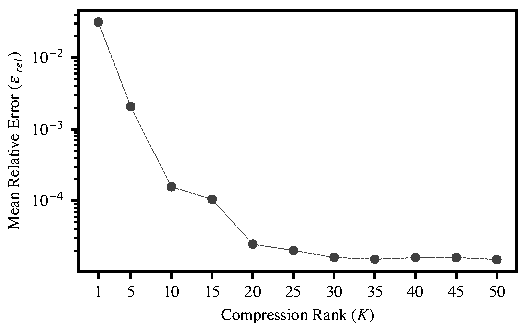
\includegraphics[width=18.5pc]{figures/compression_accuracy.pdf}}
\caption{Compression Rank and accuracy}
\end{figure}

% Larger figure
% \begin{figure*}
% \centerline{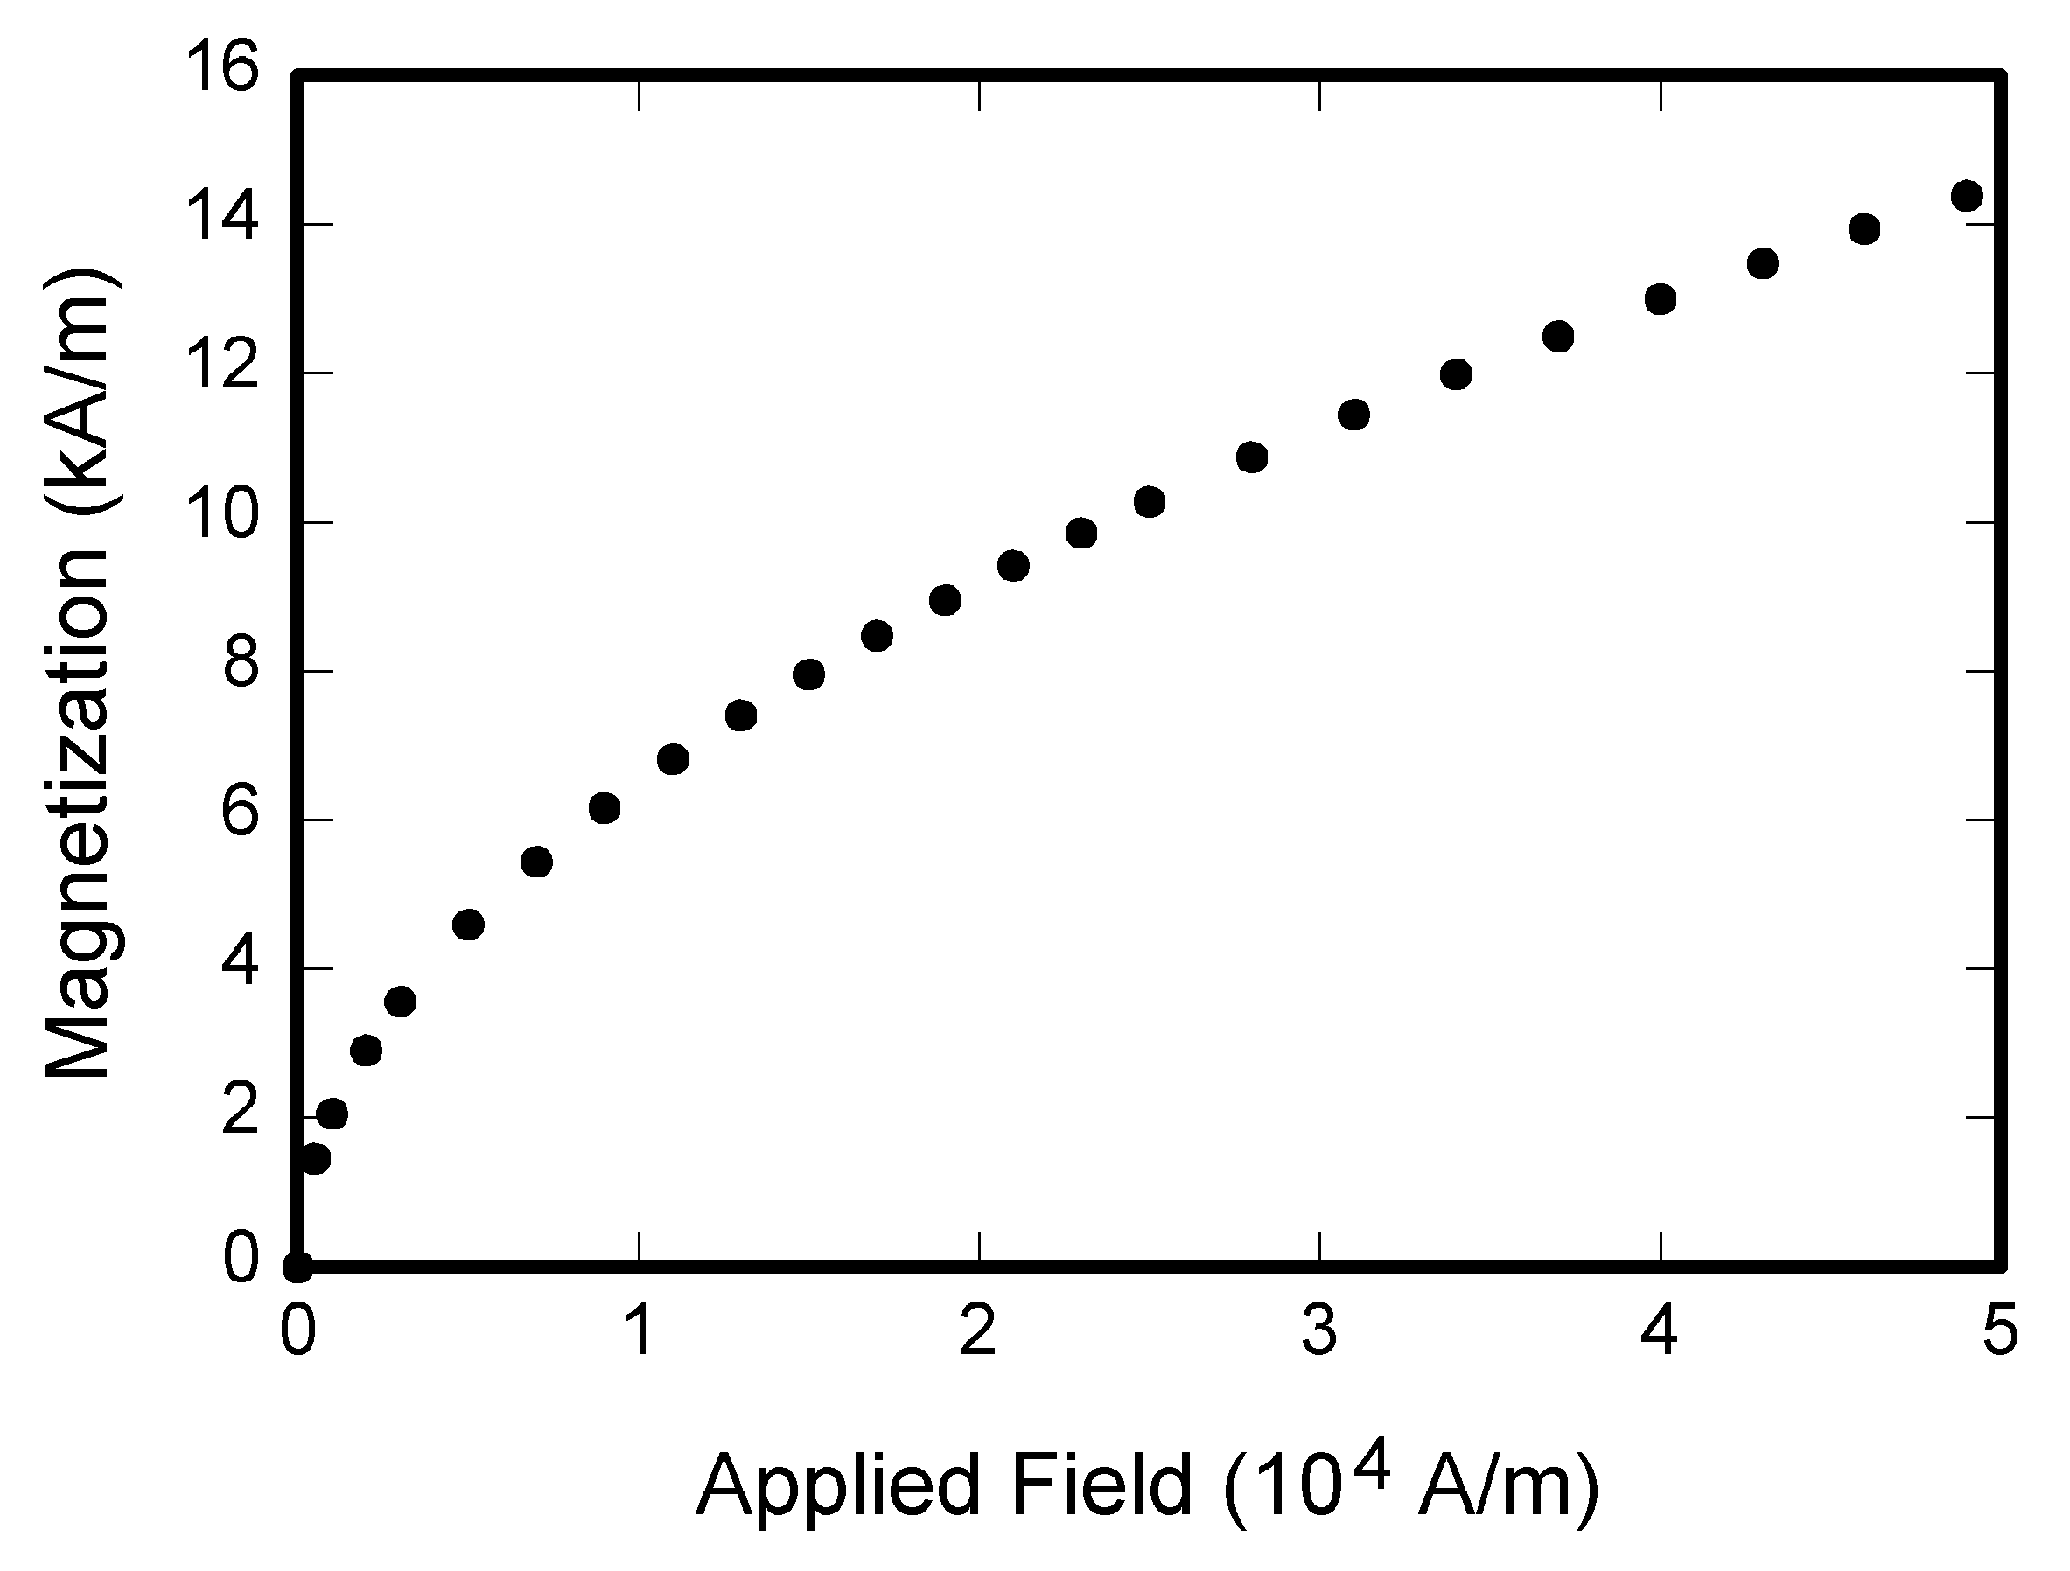
\includegraphics[width=26pc]{figures/fig1.png}}
% \caption{Note that ``Figure'' is spelled out. There is a period after the figure number, followed by one space. It is good practice to briefly explain the significance of the figure in the caption. (Used, with permission, from [4].)}
% \end{figure*}

\begin{table}
\caption{Units for magnetic properties.}
\label{table}
\small
\begin{tabular*}{17.5pc}{@{}|p{29pt}|p{63pt}<{\raggedright}|p{80pt}<{\raggedright}|@{}}
\hline
Symbol&
Quantity&
Conversion from Gaussian and  CGS EMU to SI$^{\mathrm{a}}$ \\
\hline
$\Phi $&
Magnetic flux&
1 Mx $\to  10^{-8}$ Wb $= 10^{-8}$ V $\cdot$ s \\
$B$&
Magnetic flux density,   magnetic induction&
1 G $\to  10^{-4}$ T $= 10^{-4}$ Wb/m$^{2}$ \\
$H$&
Magnetic field strength&
1 Oe $\to  10^{-3}/(4\pi )$ A/m \\
$m$&
Magnetic moment&
1 erg/G $=$ 1 emu   $\to 10^{-3}$ A $\cdot$ m$^{2} = 10^{-3}$ J/T \\
$M$&
Magnetization&
1 erg/(G $\cdot$ cm$^{3}) =$ 1 emu/cm$^{3}$   $\to 10^{-3}$ A/m \\
4$\pi M$&
Magnetization&
1 G $\to  10^{-3}/(4\pi )$ A/m \\
$\sigma $&
Specific magnetization&
1 erg/(G $\cdot$ g) $=$ 1 emu/g $\to $ 1 A $\cdot$ m$^{2}$/kg \\
$j$&
Magnetic dipole   moment&
1 erg/G $=$ 1 emu   $\to 4\pi \times  10^{-10}$ Wb $\cdot$ m \\
$J$&
Magnetic polarization&
1 erg/(G $\cdot$ cm$^{3}) =$ 1 emu/cm$^{3}$  $\to 4\pi \times  10^{-4}$ T \\
$\chi , \kappa $&
Susceptibility&
1 $\to  4\pi $ \\
$\chi_{\rho }$&
Mass susceptibility&
1 cm$^{3}$/g $\to  4\pi \times  10^{-3}$ m$^{3}$/kg \\
$\mu $&
Permeability&
1 $\to  4\pi \times  10^{-7}$ H/m   $= 4\pi \times  10^{-7}$ Wb/(A $\cdot$ m) \\
$\mu_{r}$&
Relative permeability&
$\mu \to \mu_{r}$ \\
$w, W$&
Energy density&
1 erg/cm$^{3} \to  10^{-1}$ J/m$^{3}$ \\
$N, D$&
Demagnetizing factor&
1 $\to  1/(4\pi )$ \\
\hline
\multicolumn{3}{@{}p{17.5pc}@{}}{Vertical lines are optional in tables. Statements that serve as captions for
the entire table do not need footnote letters. }\\
\multicolumn{3}{@{}p{17.5pc}@{}}{$^{\mathrm{a}}$Gaussian units are the same as cg emu for magnetostatics; Mx
$=$ maxwell, G $=$ gauss, Oe $=$ oersted; Wb $=$ weber, V $=$ volt, s $=$
second, T $=$ tesla, m $=$ meter, A $=$ ampere, J $=$ joule, kg $=$
kilogram, H $=$ henry.}
\end{tabular*}
\label{tab1}
\end{table}


\section{CONCLUSION}

What have we learned, what will we be working on next?

\section{ACKNOWLEDGMENT}

SK is supported by EPSRC Studentship 2417009.

\bibliography{pyexafmm}
\bibliographystyle{ieeetr}

\begin{IEEEbiography}{Srinath Kailasa}{\,} is a graduate student at University College London. He is currently pursuing a PhD in Computational Mathematics, having received an MPhys in Physics (2017) and an MSc Scientific Computing (2020) from the University of Durham, and University College London respectively. His research interests are in high-performance and scientific computing. Contact him at srinath.kailasa.18@ucl.ac.uk.
\end{IEEEbiography}

\begin{IEEEbiography}{Timo Betcke}{\,}is a Professor of Computational Mathematics at University College London. Contact him at t.betcke@ucl.ac.uk.
\end{IEEEbiography}

\begin{IEEEbiography}{Tingyu Wang}{\,}is a PhD student in Mechanical Engineering at the George Washington University. Contact him at twang66@email.gwu.edu.
\end{IEEEbiography}

\begin{IEEEbiography}{Lorena. A. Barba}{\,}is a Professor of Mechanical and Aerospace Engineering at the George Washington University.  Contact her at labarba@email.gwu.edu.
\end{IEEEbiography}

\end{document}

